%
% Niniejszy plik stanowi przykład formatowania pracy magisterskiej na
% Wydziale MIM UW.  Szkielet użytych poleceń można wykorzystywać do
% woli, np. formatujac wlasna prace.
%
% Zawartosc merytoryczna stanowi oryginalnosiagniecie
% naukowosciowe Marcina Wolinskiego.  Wszelkie prawa zastrzeżone.
%
% Copyright (c) 2001 by Marcin Woliński <M.Wolinski@gust.org.pl>
% Poprawki spowodowane zmianami przepisów - Marcin Szczuka, 1.10.2004
% Poprawki spowodowane zmianami przepisow i ujednolicenie
% - Seweryn Karłowicz, 05.05.2006
% Dodanie wielu autorów i tłumaczenia na angielski - Kuba Pochrybniak, 29.11.2016

% dodaj opcję [licencjacka] dla pracy licencjackiej
% dodaj opcję [en] dla wersji angielskiej (mogą być obie: [licencjacka,en])
\documentclass[licencjacka]{pracamgr}

\usepackage{hyperref}
\usepackage{graphicx}
\usepackage{listings}
\usepackage{xcolor}
\usepackage{textcomp}
\usepackage{wrapfig}
\usepackage{multirow}
\usepackage{tabularx}
\newcolumntype{R}{>{\raggedleft\arraybackslash}X}


\lstset{
  aboveskip=3mm,
  belowskip=3mm,
  showstringspaces=false,
  columns=flexible,
  basicstyle={\small\ttfamily},
  numberstyle=\tiny\color{gray},
  keywordstyle=\color{blue},
  commentstyle=\color{dkgreen},
  stringstyle=\color{mauve},
  breaklines=true,
  breakatwhitespace=true,
  tabsize=4,
  escapeinside=``,
  frame=tb
}

% Dane magistrantów:
\autori{Michał Borkowski}{370727}
\autorii{Jakub Bujak}{370737}
\autoriii{Marian Dziubiak}{370784}
\autoriv{Marek Puzyna}{371359}

\title{Kompilacja NianioLanga do efektywnych konstrukcji języka C}


%\tytulang{An implementation of a difference blabalizer based on the theory of $\sigma$ -- $\rho$ phetors}

%kierunek:
% - matematyka, informacyka, ...
% - Mathematics, Computer Science, ...
\kierunek{informatyka}

% informatyka - nie okreslamy zakresu (opcja zakomentowana)
% matematyka - zakres moze pozostac nieokreslony,
% a jesli ma byc okreslony dla pracy mgr,
% to przyjmuje jedna z wartosci:
% {metod matematycznych w finansach}
% {metod matematycznych w ubezpieczeniach}
% {matematyki stosowanej}
% {nauczania matematyki}
% Dla pracy licencjackiej mamy natomiast
% mozliwosc wpisania takiej wartosci zakresu:
% {Jednoczesnych Studiow Ekonomiczno--Matematycznych}

% \zakres{Tu wpisac, jesli trzeba, jedna z opcji podanych wyzej}

% Praca wykonana pod kierunkiem:
% (podać tytuł/stopień imię i nazwisko opiekuna
% Instytut
% ew. Wydział ew. Uczelnia (jeżeli nie MIM UW))
\opiekun{mgr. Radosława Bartosiaka\\
  Instytut Informatyki\\
  }

% miesiąc i~rok:
\date{Czerwiec 2018}

%Podać dziedzinę wg klasyfikacji Socrates-Erasmus:
\dziedzina{
%11.0 Matematyka, Informatyka:\\
%11.1 Matematyka\\
%11.2 Statystyka\\
11.3 Informatyka\\
%11.4 Sztuczna inteligencja\\
%11.5 Nauki aktuarialne\\
%11.9 Inne nauki matematyczne i informatyczne
}

%Klasyfikacja tematyczna wedlug AMS (matematyka) lub ACM (informatyka)
\klasyfikacja{D. Software\\
  D.3. Programming languages\\
  D.3.3. Language contructs and features}

% Słowa kluczowe:
\keywords{kompilacja, języki programowania, analiza semantyczna,
  NianioLang, system typów}

% Tu jest dobre miejsce na Twoje własne makra i~środowiska:
\newtheorem{defi}{Definicja}[section]

% koniec definicji

\begin{document}

\maketitle

%tu idzie streszczenie na strone poczatkowa
\begin{abstract}
W pracy opisany został proces projektowania i implementacji rozszerzenia języka NianioLang mającego umożliwić
kompilację jego zmiennych do efektywnych konstrukcji języka C przy zachowaniu jego podstawowych cech.
W pierwszej części pracy zawarte zostało wprowadzenie do języka NianioLang i stan kompilatora zastany w chwili
rozpoczynania projektu. W dalszych rozdziałach zostały opisane zmiany w systemie typów, jakie były potrzebne
do osiągnięcia zamierzonych celów i sposób implementacji tych zmian w kompilatorze.
\end{abstract}

\tableofcontents
%\listoffigures
%\listoftables

\chapter*{Wprowadzenie}
  \addcontentsline{toc}{chapter}{Wprowadzenie}
  NianioLang jest językiem programowania ogólnego przeznaczenia. Jego twórcą jest
  założyciel firmy Atinea, na zlecenie której realizowana jest poniższa
  praca -- Andrzej Gąsienica-Samek.
  Istniejący kompilator umożliwia translację NianioLanga do kilku języków,
  między innymi do Javy, JavaScriptu i C.
  Ze względu na chęć uproszczenia kompilacji NianioLanga
  utworzono środowisko uruchomieniowe dostarczające odpowiednie abstrakcje
  i pozwalające na korzystanie w C z dynamicznych struktur odpowiadających typom,
  jakie są dostępne do użycia w NianioLangu. Takie rozwiązanie nie jest
  niestety optymalne, szczególnie w przypadku niskopoziomowego języka jakim
  jest C. W tej pracy opisujemy wprowadzenie nowych typów danych i ich wsparcia
  w kompilatorze, co umożliwi generowanie natywnego kodu w C i znacznie
  zwiększy wydajność kompilowanych aplikacji przy zachowaniu podstawowych założeń języka.
\chapter{Wstęp}
\section{Wprowadzenie do NianioLanga}
NianioLang jest proceduralnym, imperatywnym językiem, którego celem jest
uproszczenie pisania rozproszonych aplikacji stosując wzorzec projektowy
Nianio\cite{wzorzec_nianio}.
Celem twórców języka jest dostarczenie narzędzia umożliwiającego operowanie na niemutowalnych strukturach
o semantyce zbliżonej do języków funkcyjnych, ale prostszego w użyciu.
Konstrukcje takie jak wskaźniki zostały usunięte, a w ich miejsce, w przypadku kompilacji do C,
zaimplementowano system zarządzania obiektami
w pamięci przez zliczanie referencji, aby pozbyć się jednego z najczęstszych źródeł błędów występujących przy programowaniu niskopoziomowym.
zabiegi zmniejszają wydajność języka, jendak jego twórcy założyli, że zysk z wysokopoziomowego podejścia
do pisania aplikacji jest wystarczająco duży, aby tworzenie aplikacji w NianioLangu było opłacalne.

Kompilator NianioLanga jest rozwijany przez firmę Atinea, która używa NianioLanga w swoich projektach (m.in. InstaDB.com).
Kod źródłowy kompilatora jest dostępny na platformie GitHub\cite{github_repo_nianiolang_original} na licencji MIT.

Szczegółowe informacje na temat założeń NianioLanga i jego składni można znaleźć na oficjalnej
stronie projektu\cite{nianiolang_org}.

\section{Typy w NianioLangu}
W NianioLangu mamy do czynienia z kilkoma wbudowanymi typami. Wszelkie typy tworzone przez użytkownika to w rzeczywistości aliasy na typy wbudowane,
co pomaga w zarządzaniu abstrakcją w programie. Dostępnych jest pięć wbudowanych typów: 
\begin{itemize}
  \item \texttt{ptd::sim} -- liczby całkowite, zmiennoprzecinkowe oraz ciągi znaków
  \item \texttt{ptd::rec} -- rekordy, czyli odpowiedniki struktur znanych np. z C
  \item \texttt{ptd::hash} -- słowniki o kluczach będących ciągami znaków i wartościach danego typu
  \item \texttt{ptd::var} -- typ wariantowy, który reprezentuje obiekty, mogące być w dokładnie jednym z określonego zbioru stanów i dodatkowo
  zawierać dane o typie właściwym dla danego stanu
  \item \texttt{ptd::arr} -- tablice danych tego samego typu
\end{itemize}

Typy te mogą być ze sobą łączone w bardziej skompilowane konstrukcje, na przykład \texttt{ptd::arr(ptd::sim())} definiuje
typ tablicy wartości prostych, a \texttt{ptd::rec(\{a => ptd::sim(), b => ptd::sim()\})} definiuje typ rekordu o dwóch polach będących wartościami
prostymi.

Podstawowymi założeniami systemu typów w NianioLangu są: niemutowalność struktur i opcjonalne typowanie.

\begin{itemize}
 \item Niemutowalność struktur w NianioLangu jest pojęciem słabszym, niż w językach funkcyjnych. Oznacza ona,
 że język daje gwarancję, iż między dwoma kolejnymi dostępami do zmiennej jej wartość nie ulegnie zmianie.
 W klasycznych językach imperatywnych, posiadających wskaźniki lub referencje nie jest to prawdą -- jeśli istnieją dwa wskaźniki
 do jednej zmiennej, wartość odczytana z jednego z nich może się zmieniać nawet bez jego jawnej modyfikacji.
 \item Opcjonalne typowanie oznacza gwarancję, że dodanie lub usunięcie typów z programu nie zmieni jego semantyki.
 W skrajnym przypadku można usunąć z programu całą informację o typach i będzie on działał bez zmian
 (oczywiście może to być ze szkodą dla łatwości utrzymania lub wydajności). Jest to podejście przeciwne do stosowanego
 w takich językach jak C++ czy Java, których złożone systemy typów mają istotny wpływ na semantykę programu.
\end{itemize}

W wielu językach istnieje znacznie więcej wbudowanych typów, jednak powyższe są wystarczające, by budować skomplikowane aplikacje,
a jednocześnie dość proste, by rozpoczęcie programowania w NianioLangu nie było dla programisty wyzwaniem.
W rozdziale \textit{\nameref{sec:compiler}} opisana została implementacja powyższych typów w języku C.

\section{Cele projektu}
Celem projektu była modyfikacja kompilatora NianioLanga w taki sposób, aby kod wynikowy w C zawierał mniejszą liczbę wywołań funkcji oraz
skomplikowanych
struktur dla prostych typów istniejących już w języku C.
Dzięki temu zmniejszony został czas wykonania aplikacji, pozwalając kompilatorowi GCC na zastosowanie dodatkowych optymalizacji.
W tym celu wprowadzone zostały nowe typy z przestrzeni nazw \texttt{own},
które będą bardziej niskopoziomowymi odpowiednikami typów z przestrzeni nazw \texttt{ptd} (rekordy, tablice i warianty).
Dzięki nałożonym na nie ograniczeniom możliwe jest znaczne zwiększenie wydajności programów pisanych w NianioLangu przy zachowaniu
niezmienionej semantyki języka.
Jednocześnie zmienione zostały pewne podstawowe typy, mianowicie \texttt{ptd::sim} został rozbity na
\texttt{ptd::int} oraz \texttt{ptd::string}, oraz wprowadzony został typ \texttt{ptd::bool}.
Liczby całkowite i wartości boolowskie mają w języku C natywną reprezentację i używając ich bezpośrednio
uzyskujemy prostszy kod wynikowy w C, który jest łatwiejszy do optymalizacji przez kompilator GCC.

Skutkiem zmian jakie musiały zostać wprowadzone by osiągnąć cel projektu było utracenie możliwości
kompilacji NianioLanga do języków innych niż C do czasu implementacji nowych typów w pozostałych językach.
To zadanie pozostaje jednak poza zakresem niniejszej pracy.

\section{Podstawowe pojęcia}
Jesli nie zaznaczono inaczej, pojęcia dotyczące kompilacji rozumiane są zgodnie z definicjami
podanymi w książce\cite{dragonbook}. W przypadku poniższych pojęć posługujemy się podanymi niżej definicjami, gdyż w bardziej naturalny sposób oddają sposób funkcjonowania kompilatora.
\begin{itemize}
  \item[] \textbf{AST} (ang. \textit{abstract syntax tree}) -- drzewo składni abstrakcyjnej,
    reprezentacja programu w formie drzewa, w którym każdy węzeł
    reprezentuje konstrukcję języka, a jego synowie reprezentują części składowe tej konstrukcji
  \item[] \textbf{nlasm} -- język maszyny rejestrowej, będący językiem pośrednim w kompilatorze NianioLanga
  \item[] \textbf{parsowanie, analiza składniowa} -- proces przetwarzania kodu źródłowego programu na równoważne drzewo
  AST
  \item[] \textbf{analiza semantyczna} -- proces sprawdzania programu na poziomie znaczenia poszczególnych instrukcji
  oraz zbierania informacji potrzebnych na kolejnych etapach
  \item[] \textbf{translacja} -- proces tłumaczenia drzewa AST na język pośredni
  \item[] \textbf{generowanie} -- proces tłumaczenia języka pośredniego na język docelowy
\end{itemize}

\chapter{Metodyka pracy}
Prace nad kodem prowadzone były regularnie od połowy października 2017 do maja 2018,
z wyłączeniem sesji na przełomie lutego i stycznia. Na rysunku \ref{img:commits_over_time}
przedstawiony został wykres zmian, które wpływały na główną gałąź repozytorium kodu.
Co tydzień zespół prezentował swoje poczynania opiekunowi, co dostarczało stałej motywacji
do implementacji kolejnych elementów projektu.

\begin{figure}[h]
  \centering
  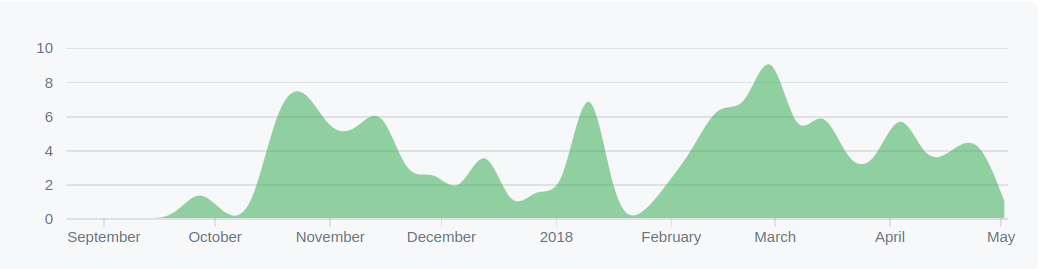
\includegraphics[width=0.9\textwidth]{files/commits_over_time}
  \caption{Liczba commitów na głównej gałęzi repozytorium w czasie trwania projektu.}
  \label{img:commits_over_time}
\end{figure}

\section{Programowanie zwinne}
Metodyka pracy, z której korzystaliśmy, najbliższa była metodyce programowania zwinnego (ang. \textit{agile}).
Praca toczyła się w iteracjach, a każda iteracja dostarczała implementację nowego typu.
Fragmenty kodu NianioLanga korzystające z tych typów oraz odpowiadające im pogramy wynikowe w języku
C były na bieżąco przesyłane do zleceniodawcy i konsultowane z nim.

Metodyka ta została wybrana ze względu na brak jasnego początkowego zakresu pracy.
Praca nad językiem miała charakter badawczy i wymagała zdefiniowania semantyki nowych typów,
która ulegała ciągłym zmianom w tracie trwania projektu.
Dzięki ciągłej konsulatcji ze zleceniodawcą można było na bieżąco wykrywać problemy z definicją typów
i szybko na nie reagować.


\section{Korzystanie z systemu kontroli wersji}
Podczas pracy zespołowej niezmiernie istotna jest wymiana i zarządzanie fragmentami kodu,
jakie piszą poszczególni członkowie zespołu. Ponieważ każdy w zespole pracował już
wcześniej z systemem kontroli wersji Git, został on użyty w tym projekcie.
Dodatkowym atutem tego systemu kontroli wersji jest szeroka dostępność darmowych
publicznych repozytoriów kodu online. Kod projektu umieszczony został na portalu
GitHub, który jest największym serwisem pozwalającym na hostowanie kodu online.

Początkowo każdy w zespole miał swoją gałąź w repozytorium, oznaczoną jego imieniem,
na której wprowadzał swoje zmiany. Jednak w trakcie pracy za praktyczniejsze podejście
zostało uznane tworzenie osobnych gałęzi kodu dla każdego zadania.
Umożliwiło to pracę nad kilkoma niezależnymi zadaniami jednocześnie i ułatwiło
przeglądy kodu poprzez tematyczny podział zmian.

GitHub, oprócz repozytorium kodu, udostępnia również narzędzia do zarządzania zadaniami
w projekcie, co zostało wykorzystane. Każde duże i średnie zadanie było zapisywane
w systemie zgłoszeń. Po ustaleniu osoby wykonującej zadanie było ono przypisywane
na tę osobę, a po wgraniu zmian na główną gałąź zamykane.
Dzięki temu w dowolnej chwili możliwe było określenie nad czym pracuje dany członek
zespołu i jakie otwarte zadania pozostały do przydzielenia.

\section{Zgłaszanie zmian i code review}
Po napisaniu kodu rozwiązującego dane zadanie zgłaszany był tzw. pull request,
czyli żądanie zatwierdzenia zmian. Aby zmiany zostały zatwierdzone i umieszczone
w głównej gałęzi projektu musiały być zatwierdzone przez co najmniej jednego członka
zespołu, innego niż ten, który zgłosił pull request. GitHub udostępnia widok naniesionych zmian
wraz z możliwością dodawania komentarzy do konkretnych fragmentów kodu. Możliwy więc
był dialog między recenzentem kodu a jego twórcą tak, aby ostatecznie zatwierdzone
zmiany spełniały oczekiwania obu stron.

\section{Testowanie i ciągła integracja}
W projekcie została wykorzystana praktyka ciągłej integracji z wykorzystaniem systemu Travis.
Został on wybrany, ponieważ jest dostępny bez dodatkowych kosztów i umożliwia łatwą integrację z repozytorium kodu
na platformie GitHub.

Każdorazowo po przesłaniu zmian do repozytorium uruchamiany był skrypt sprawdzający, czy dana wersja kompilatora
kompiluje się i przechodzi szereg testów automatycznych.
Zmiany, w wyniku których program nie przechodził weryfikacji testami, nie mogły być scalane z główną gałęzią.

Testy na początku projektu obejmowały całość istniejącego języka.
Za każdym razem, kiedy były dodawane nowe typy lub nowe operacje na już istniejących typach,
testy były uzupełnianie o daną konstrukcję.
W ten sposób można było łatwo sprawdzić, czy nowe zmiany nie wpłynęły negatywnie na działające wcześniej funkcje.

\section{Techniki komunikacji w zespole}
Większość komunikacji w zespole odbywała się online przez portal społecznościowy Facebook.
W początkowej fazie projektu głównym tematem dyskusji była specyfika języka NianioLang,
z którym większość członków zespołu miała po raz pierwszy styczność.
Na dalszym etapie projektu, przy użyciu konwersacji grupowej na tym portalu, zespół
ustalał większość detali implementacyjnych przed rozpoczęciem ich wdrażania.
Ten środek komunikacji był najchętniej wykorzystywany ze względu na najkrótszy czas
reakcji członków zespołu.

Drugim kanałem komunikacji były zadania i pull requesty na GitHubie. Zadania w prosty sposób
opisywały przydział i zakres, a opisy pull requestów określały, co zostało przez daną osobę zrobione.

Ostatnim sposobem komunikacji były cotygodniowe spotkania podczas zajęć z Zespołowego
Projektu Programistycznego, po których członkowie zespołu spędzali chwilę na ustalaniu
szczegółów planu pracy przez kolejny tydzień, a w przypadku pytań lub problemów, na ich rozwiązaniu.

\chapter{Kompilator NianioLanga}
\label{sec:compiler}
\section{Budowanie drzewa AST}
Pierwszym etapem kompilacji jest parsowanie programu wejściowego do drzewa AST. Takie drzewo jest strukturą przechowującą informacje o składniowej
roli wyrażeń, które przetwarzać można na dalszych etapach kompilacji. Celem jest przetworzenie tekstu programu do postaci przypominającej derywację
gramatyki języka. Chociaż książkowa definicja drzewa AST mówi wyłącznie o składni, kompilator NianioLanga już na tym etapie dokonuje pewnej
podstawowej analizy semantycznej, gdyż wydzielenie tych czynności spowodowałoby dużą duplikację kodu związanego z czynnością obchodzenia drzewa.

\begin{figure}[h]
  \centering
  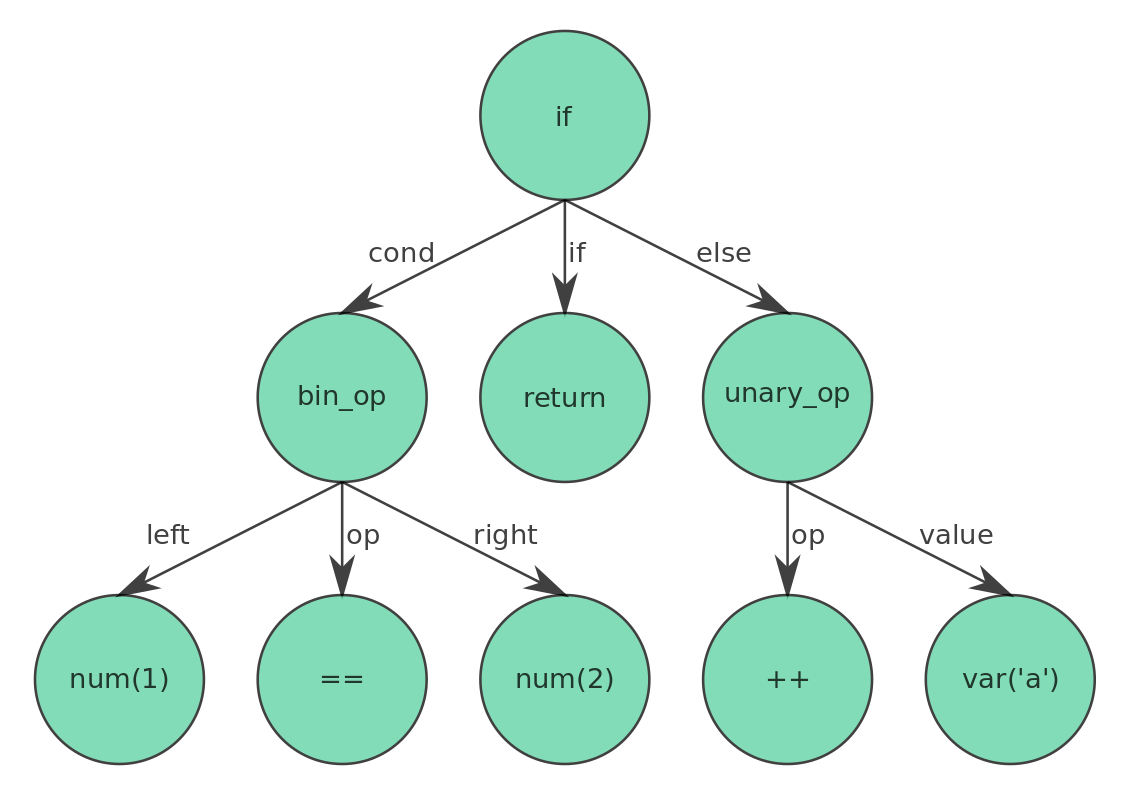
\includegraphics[width=0.6\textwidth]{files/ast.png}
  \caption{Drzewo AST dla programu \texttt{if (1 == 2) \{return;\} else \{a++;\}}}
  \label{img:ast}
\end{figure}

Najpierw parser próbuje przeczytać listę importowanych modułów, gdyż zgodnie ze składnią języka musi ona zostać umieszczona na początku programu. Po
tym etapie następuje parsowanie listy funkcji. Każdy etap parsowania odbywa się poprzez analizę możliwie najdłuższego fragmentu tekstu, dopisanie błędów,
ustawienie wskaźnika następnej pozycji oraz innych pomocniczych wartości, które są przechowywane w zmiennej reprezentującej stan parsera, a na końcu
zwrócenie sparsowanej wartości. Nie ma znaczenia, co zwróci dana funkcja w razie błędu, gdyż wtedy kompilacja zostanie zatrzymana, a użytkownik
poinformowany o błędzie. W przypadku, gdy nie jest jasne, co należy sparsować (na przykład nie wiadomo, czy oczekujemy kolejnej deklaracji importu
modułu, czy definicji funkcji), próbuje się przeczytać różne wartości, aż któraś zostanie poprawnie sparsowana. Ważne jest, by różne możliwości
przetwarzać od największej do najmniejszej, jeżeli reprezentacja jedna może być początkiem drugiej, np. najpierw parsować należy operatory, a dopiero
potem wyrażenia, chyba że kolejność nie ma znaczenia. Przykładowo w wyrażeniu \emph{1 + 2 - 3} nie ma znaczenia, czy spróbujemy sparsować najpierw
operator dodawania, czy odejmowania, ale operator musi być sparsowany zanim sparsowana zostanie liczba. Innym przykładem jest \texttt{if}, po którym
może nastąpić \texttt{else} i najpierw należy spróbować sparsować blok \texttt{else} zanim przejdzie się do parsowania następnych komend.

Parsowanie funkcji odbywa się poprzez sparsowanie nagłówka, a następnie sparsowanie jej wnętrza jako jednej komendy. Przyjęte jest, że komenda może
być także listą komend, co parsuje się w sposób rekurencyjny. Ułatwia to parsowanie takich komend jak \texttt{for} czy \texttt{if}. Podejście to
umożliwia także tworzenie rekurencyjnych funkcji, z których każda odpowiedzialna jest za jeden element gramatyki języka. Funkcje te sposób działania
opierają na opisanym w poprzednim paragrafie schemacie.

Projekt nie wymagał znaczących zmian na etapie parsowania, dlatego nie zostaną one tutaj omówione. Jedynym wyjątkiem jest dodanie sprawdzania po
sparsowaniu funkcji, czy nie definiuje ona typu, a następnie wpisania tego typu do drzewa. Zostało to jednak wykonane przy użyciu dostępnych już
funkcji. Jest to wykonywane, by na dalszych etapach można było zapytać o dowolny definiowany typ, co ułatwia proces kompilacji. Sytuacja błędna nie
jest jednak obsługiwana, stanie się to dopiero podczas sprawdzania poprawności typów.
\section{Analiza semantyczna}
Drugim etapem kompilacji jest sprawdzenie poprawności typów. Wbrew nazwie etap ten nie ma na celu wyłącznie sprawdzenia, czy program jest poprawny
typowo -- do drzewa programu wpisywane są informacje o uzyskanych typach. Jest to konieczne, by móc dopasować typy NianioLanga do typów języka
wynikowego. Ponadto zachodzi tutaj analiza opisana w rozdziale \textit{\nameref{sec:own_to_im}}.

Na tym etapie sprawdza się, czy zaimportowane moduły faktycznie istnieją, czy definicje funkcji nie dublują się, oraz w końcu czy używane typy zgodne
są z oczekiwanymi. Trzeci element rozumiany jest dwojako. Po pierwsze, jeżeli dana zmienna ma zadeklarowany przez użytkownika typ, sprawdza się, czy
używana jest ona wyłącznie przez funkcje, które takiego typu oczekują.  Ze względu na nietrywialny system typów wydzielone są specjalne funkcje
sprawdzające czy i w jakim zakresie dwa typy są zgodne. Przykładowo jeżeli \texttt{im} używany jest w kontekście \texttt{hash}, to zgodnym typem jest
\texttt{hash}. Jeżeli zaś funkcja oczekuje \texttt{int} a podawany jest \texttt{array}, to zgłaszany jest błąd. W czasie działania tej części kompilatora o typach myśleć można
jako o zbiorach możliwych wartości, na których wykonywane są operacje, przede wszystkim przecięcia.

Drugie rozumienie, które stosuje type checker, jest podobne do pierwszego, lecz w kontekście wnioskowania typów na podstawie wykonywanych na nich
operacji. Jeżeli dana zmienna inicjalizowana jest jako \texttt{int}, a następnie używana jako \texttt{hash}, to zgłaszany jest błąd. Warto zaznaczyć,
że operacje na typach wywnioskowanych są subtelniejsze, gdyż wiele typów jest konwertowalnych na \texttt{im} oraz w drugą stronę, przez co nie jest
możliwa całkowita, ścisła kontrola typów, ta ma miejsce dopiero w runtime. Ponownie, wydzielone są funkcje operujące na typach w analogii do zbiorów.

Samą budowę type checker ma podobną w pewnym sensie do parsera. W rekurencyjny sposób sprawdzamy, jakie typy mają poszczególne elementy drzewa oraz
czy są one poprawne. Tak jak w parserze zapisane jest, że operator \texttt{+} zawiera słowo kluczowe \texttt{+}, tak odpowiednia funkcja w type
checkerze wie, że argumenty tego operatora muszą mieć typ zwracany \texttt{int}. Ponownie pozwala to na podział funkcji w taki sposób, by każda
dotyczyła jednego, jasno wyszczególnionego elementu.
\section{Architektura nlasma}
nlasm to język stosowany w kompilatorze jako język pośredni pomiędzy NianioLangiem a językiem docelowy.
Został wprowadzony, gdyż bezpośrednia kompilacja NianioLanga do C, lub
też innego języka, może okazać się trudna, ponieważ używane struktury językowe znacząco od siebie odbiegają. Umożliwia to w łatwy sposób tworzenie
modułów kompilujących NianioLanga do różnych języków. Taka technika jest szeroko stosowana w świecie kompilatorów, jednym z najszerzej znanych
przykładów jest LLVM. Obecność autorskiego nlasma podyktowana jest przede wszystkim potrzebą języka pośredniego, który z jednej strony będzie możliwie
najprostszy, z drugiej w pewnym sensie zachowa strukturę programu wyjściowego.

Funkcje w nlasmie nie operują na zmiennych, lecz na rejestrach. Każdy rejestr ma swój unikalny w obrębie funkcji numer oraz typ. Także argumenty
funkcji są rejestrami. Wprowadzenie typów do nlasma było jednym z elementów projektu, gdyż o ile poprzednio wszystkie zmienne konwertowane były do
typu \texttt{im}, o tyle teraz przechować należy strukturę typów \texttt{own} czy \texttt{int}. Typy w nlasmie mają charakter wyłącznie informacyjny,
to znaczy nie mają żadnego znaczenia semantycznego. Są używane na dalszych etapach kompilacji.

Najważniejszą cechą nlasma jest nie drzewiasta, lecz liniowa struktura programu. Oznacza to, że argumentami wywołań mogą być wyłącznie rejestry, a nie
zmienne czy inne wywołania. W znacznym stopniu ułatwia to dalszą pracę kompilatora, przede wszystkim z powodu mniejszej liczby problemów dotyczących na
przykład wartości zwracanych, przez co kod generatora języka docelowego może być znacznie prostszy. Ponadto generowanie kodu może odbywać się w sposób
liniowy, to znaczy każda komenda nlasma może mieć jednoznaczne, proste odzwierciedlenie w języku docelowym. Dzięki temu generator może dokonywać
analizy wyłącznie w zakresie charakterystycznym dla danego języka, na przykład do generatora C zostało wprowadzone sortowanie topologiczne deklaracji
typów.

Inną ważną cechą nlasma, wynikającą częściowo z poprzedniej, jest brak pętli. Translator NianioLanga do nlasm musi rozbić każdą pętlę na etykietę oraz
komendę \texttt{goto}. Takie podejście ułatwia tłumaczenie kodu na język docelowy, gdyż w różnych językach pętle działają w odrobinę inny sposób, zaś
\texttt{goto} tworzy nieskomplikowany, wspólny interfejs.

Ponadto nlasm zawiera polecenia służące do zarządzania pamięcią. Zakłada się, że język docelowy będzie korzystał ze zliczania referencji w celu
zwalniania pamięci. Aby nie pisać tej samej funkcjonalności oddzielnie dla wielu generatorów, nlasm zawiera polecenia mówiące o tym, że licznik
referencji danego rejestru (o ile jest on wskaźnikiem) należy zmniejszyć lub zwiększyć, co można w prosty sposób przełożyć na wywołania innych
języków. Oczywiście, jeżeli generator wybierze inną metodę zarządzania pamięcią, na przykład generując kod Javy, może te polecenia po prostu
zignorować. W przypadku generowania języka z manualnym zarządzaniem pamięcią, na przykład C, polecenia te są bardzo pomocne.


Przykładowe komendy nlasma:
\begin{itemize}
\item \texttt{if\_goto} -- sprawdza wartość w rejestrze. Jeżeli prawda, wykonuje skok pod etykietę
\item \texttt{clear} -- sygnalizuje, że wartość licznika referencji powinna spaść
\item \texttt{call} -- wywołuje funkcję o danej nazwie z danymi rejestrami jako argumentami, zapisuje wynik w danym rejestrze
\item \texttt{move} -- kopiuje wartość między dwoma rejestrami
\end{itemize}
\section{Translacja drzewa AST do nlasma}
\label{sec:translation}
Drzewo AST, reprezentujące funkcję języka nianiolang, jest w sposób rekurencyjny tłumaczone na ciąg komend nlasma. Sposobem działania 
komendy nlasma przypominają rozkazy maszynowe: identyfikator komendy + identyfikatory rejestrów. Zgodnie ze specyfikacją języka nlasm, każdemu argumentowi funkcji, jak 
i każdej zmiennej lokalnej, jest przydzielany rejestr odpowiedniego typu. Ze względu na strukturę języka nlasm brak w nim jakichkolwiek rozgałęzień kodu, 
więc każda instrukcja warunkowa czy pętla jest tłumaczona na odpowiedni ciąg komend, zawierający warunkowy skok (komendę \texttt{if\_goto}) do 
odpowiedniej etykiety. Przypisanie wartości jednej zmiennej do innej jest realizowane za pomocą komendy \texttt{move}. 

Tłumaczenie wartości wyrażeń jest bardziej skomplikowane: dla danego wierzchołka w drzewie AST generujemy wywołania komend obliczające wartości w 
danym wierzchołku na podstawie podwyrażeń. Na przykład dla wyrażeń arytmetycznych zapisujemy wartości lewej i prawej strony w odpowiednich rejestrach, po czym 
stosujemy komendę \texttt{bin\_op}, która dla danych trzech rejestrów: docelowego, lewej strony i prawej strony wyrażenia, a także operatora, oblicza 
wartość i zapisuje w odpowiednim rejestrze. Dla operacji posiadających skutki uboczne (np. zapisanie wartości do zmiennej) stosujemy tzw. obliczanie 
z powrotem: jeśli obliczany operator zapisuje pewną wartość do lewej części wyrażenia, która w takim przypadku powinna być zmienną bądź ciągiem 
dostępów do elementów talic/haszy/rekordów kończącym się wartością, oblicza on ciąg zstępujący odwołań do elementów kolekcji. To translator realizuje za 
pomocą wywołań określonych funkcji bibliotecznych: \texttt{get\_ref\_arr}, \texttt{get\_ref\_hash}, wywołując je z odpowiednimi parametrami za pomocą 
komendy \texttt{call}, bądź, w przypadku rekordów, za pomocą komendy \texttt{key}. Funcje te tworzą kopię elementu kolekcji, którą zapisują w 
odpowiednim rejestrze. Po zapisaniu nowej wartości translator generuje ciąg przypisań elementów do ich pozycji w kolekcji za pomocą komend 
\texttt{set\_at\_idx}, \texttt{set\_val}. Na przykład, tłumacząc operatory arytmetyczne, przypisujące wynik do lewej strony (np. \texttt{+=}), na 
początek obliczamy ciąg dostępów do wartości lewej strony, obliczamy prawą stronę, wynik, po czym generuje się ciąg przypisań nowych wartości dla odpowiednich elementów kolejnych 
kolekcji.

\section{Generowanie kodu C na podstawie nlasma}
Jak zostało to omówione w poprzednim rozdziale, nlasm został zaprojektowany z myślą o ułatwieniu dalszej kompilacji. Wobec tego generowanie
kodu C jest bardzo proste.


Pierwszym etapem jest wygenerowanie kodu dla pliku nagłówkowego modułu. Zawiera on między innymi komentarz z informacją o tym, że dany plik został
wygenerowany automatycznie, instrukcje importujące nagłówki C biblioteki standardowej NianioLanga, czy też pewne instrukcje inicjujące, na przykład
ustawiające wartości stałych. Warto wspomnieć, że pliki \texttt{.c} i \texttt{.h} generowane są równolegle, gdyż pozwala to na przetwarzanie zgodnie z
kolejnością semantyczną, to znaczy na przykład generowanie wszelkich informacji o funkcji można oddelegować do raz wywoływanej procedury.


Drugim etapem jest wygenerowanie kodu odpowiedzialnego za obsługę typów, czyli ich deklaracje, definicje, oraz potrzebne do obsługi funkcje. Przed
zmianami wprowadzonymi w ramach tego projektu etap ten nie występował, gdyż kod C używał ogólnego typu \texttt{ImmT}, który obsługiwać można
biblioteką standardową NianioLanga. Obecnie, ponieważ dla każdego typu \texttt{own} tworzony jest oddzielny typ na poziomie C, a funkcje go
obsługujące generowane są na poziomie NianioLanga, to podejście zostało zmienione. Ze względu na fakt, że definicje w NianioLangu nie muszą występować
w określonej kolejności, lecz w C już tak, konieczne jest sortowanie topologiczne, z uwzględnieniem możliwości wyodrębnionej deklaracji typu. Jest to
potrzebne do obsługi sytuacji, w której typ \texttt{A} potrzebuje w swojej definicji posługiwać się w pełni typem \texttt{B}, który z kolei posługuje
się wskaźnikiem na typ \texttt{A}.


Trzecim i ostatnim etapem jest wygenerowanie kodu odpowiedzialnego za same funkcje NianioLanga. Komendy nlasm w bardzo prosty sposób tłumaczą się na
język C.
Wobec tego generator na tym etapie wykonuje jedynie pracę związaną z właściwie słownikowym przełożeniem instrukcji,
mając jedynie na uwadze pewne szczegóły techniczne. Do tych szczegółów należy, pośród innych pomniejszych zadań, utworzenie wrapperów na funkcje tak,
by można było je wywoływać także mając daną tablicę argumentów, obsługa wskaźników i zarządzanie pamięcią oraz tworzenie komentarzy będących
informacją, której linii oryginalnego programu odpowiada dana seria instrukcji.


Po wykonaniu wszystkich trzech etapów pliki \texttt{.c} i \texttt{.h} danego modułu gotowe są do zapisania na dysku, a kompilator przechodzi do
tłumaczenia kolejnego modułu.
\section{Implementacja typów NianioLanga w C}
\label{sec:c_types_implementation}
Implementacja typów \texttt{ptd} opiera się na generycznym typie \texttt{ImmT}. Typ ten zdefiniowany jest jako \texttt{void*}, a w czasie wykonania
programu wskazuje na konkretne struktury danego obiektu. Pierwsze bajty każdego obiektu zawierają informacje o tym, jaki jest jego typ, oraz jaką
wartość ma licznik referencji. Jest to powszechny schemat symulowania programowania obiektowego w językach, które takowego nie wspierają, a takim
językiem jest C.

Operacje na danych definiowane są przez szereg funkcji dostępnych w bibliotece standardowej NianioLanga, dokompilowywanej do każdego programu, to
znaczy każdy moduł NianioLanga importuje jej nagłówki. Zawierają one podstawową funkcjonalność obsługi arytmetyki, struktur danych, operacji I/O.

Cała obsługa jest dość prosta i ma charakter możliwie najbardziej generyczny, wobec czego jest niezwykle niewydajna, w szczególności w kontekście
operacji na liczbach lub wartościach logicznych.
Przed wykonaniem dowolnej operacji na zmiennej o którymś z tych typów konieczne jest odpakowanie konkretnej wartości
ze zmiennej, wykonanie na niej danej operacji, a następnie opakowanie jej z powrotem w typ \texttt{ImmT}.
Szczególny problem pojawia się przy operacjach na wartościach logicznych: nie mają one bezpośredniego odzwierciedlenia
w typach NianioLanga i są zaimplementowane jako warianty o wartościach \texttt{:TRUE} lub \texttt{:FALSE}.
Każda operacja na wartościach logicznych wymaga więc, oprócz odpakowania wartości z typu \texttt{ImmT}, rozpoznania,
który z wariantów reprezentuje ta zmienna.
Stanowi to bardzo dużą różnicę w stosunku do czystych wartości logicznych języka C, na których operacje nie wymagają
całego tego narzutu.


Celem projektu była zmiana tej sytuacji i umożliwienie kompilatorowi C zastosowanie większej liczby
optymalizacji, co opisane jest w kolejnych rozdziałach.


\chapter{Zmiana systemu typów}
\section{Niezmienione cechy języka}
Z powodu dużego zakresu zmian przeprowadzonych w ramach niniejszej pracy, ważnym zadaniem było wyodrębnienie
podstawowych cech NianioLanga, które nie mogą ulec zmianie w wyniku jego rozwoju. Takimi cechami są:
\begin{itemize}
 \item Niezmienialność struktur -- wartość zmiennej nie może ulec zmianie pomiędzy dwiema kolejnymi jawnymi
 modyfikacjami
 \item Ścisła opcjonalność typów -- poprawny program po usunięciu wszystkich informacji o typach musi pozostać
 poprawny, a jego semantyka nie może się zmienić
\end{itemize}
Zachowanie powyższych cech zostało uznane za priorytet i miało wpływ na wiele podjętych podczas projektowania
decyzji.

\section{Rozdzielenie typu \texttt{ptd::sim}}
Najpoważniejszą zmianą, jaka zaszła w systemie typów w wyniku niniejszego projektu, było rozdzielenie
typu \texttt{ptd::sim} na typy \texttt{ptd::int} i \texttt{ptd::string}, oraz rezygnacja ze wsparcia
języka dla liczb zmiennoprzecinkowych. Zmiana ta niesie ze sobą duże konsekwencje, przede wszystkim łamie
ona kompatybilność wsteczną, przez co duża część dotychczas poprawnych programów nie daje się skompilować nową
wersją kompilatora. Decyzja o wprowadzeniu tej zmiany była podjęta z dwóch powodów:
\begin{itemize}
 \item Wbrew początkowym założeniom języka, semantyka typów liczb całkowitych i łańcuchów znaków
 okazała się zupełnie inna. Pierwszy z nich jest wykorzystywany do operacji arytmetycznych i indeksowania tablic,
 podczas gdy drugi służy do indeksowania tablic asocjacyjnych. Obszary ich zastosowań są w dużej części rozłączne
 i brak kontroli rzutowania pomiędzy nimi prowadzi nieraz do błędnego modelowania dziedziny, co w efekcie
 może skutkować trudnymi do wykrycia błędami.
 \item Narzut związany z przechowywaniem i sprawdzaniem typu zmiennej jest bardzo duży, zwłaszcza
 w przypadku liczb całkowitych. Rozdzielenie typu prostego na dwa typy umożliwiło generowanie bardziej
 wyspecjalizowanego kodu, co w efekcie znacząco przyspieszyło programy wynikowe.
\end{itemize}
Usunięcie obsługi liczb zmiennoprzecinkowych wynikało z analizy istniejącego kodu i było wykonane niejako
przy okazji. W trakcie analizy okazało się, że programy niemal nie korzystają z operacji na liczbach
zmiennoprzecinkowych, a ich uwzględnienie w języku znacząco komplikuje kod kompilatora. Jednocześnie,
z uwagi na łatwość integracji programów napisanych w NianioLangu z programami napisanymi w C, obsługa
liczb zmiennoprzecinkowych może zostać w razie potrzeby dodana w formie biblioteki.

\section{Typy \texttt{own}}
\subsection{Powody wprowadzenia typów \texttt{own}}
Drugą dużą zmianą wprowadzoną w systemie typów było dodanie całkiem nowej przestrzeni typów \texttt{own} obok
istniejącej przestrzeni \texttt{ptd}. Celem nowych typów jest możliwość efektywnej kompilacji do
prostych konstrukcji języka C, pozwala na generowanie efektywniejszych programów wynikowych. 

\begin{wrapfigure}[19]{r}{.5\textwidth}
\begin{lstlisting}[caption={Przykład funkcji nianio},label={lst:nianio},aboveskip=-15pt]
def nianio::state() {
    return ptd::rec({
        num => ptd::int(),
        bool => ptd::bool(),
    });
}
def nianio::nianio(ref state : @nianio::state, cmd) {
    match (cmd) case :inc_num(var inc) {
        inc_num(ref state, inc);
    } case :neg_bool {
         state->bool = !state->bool;
    }
}
def inc_num(ref state : @nianio::state, inc) {
    state->num += inc;
}
\end{lstlisting}
\end{wrapfigure}
Szczególnym przypadkiem użycia dla nowych typów jest opis stanu we wzorcu nianio.
Abstrahując od szczegółów, istotą wzorca nianio jest utrzymywanie stanu aplikacji w jednej zmiennej
i modyfikowanie go jedynie poprzez polecenia wysyłane do funkcji nianio (przykład znajduje się
na listingu \ref{lst:nianio}). W przypadku bardziej skompilowanych aplikacji o złożonym stanie,
zmienna \texttt{state} może być bardzo głęboko zagnieżdżona, a ponieważ modyfikacja liści jest najczęściej
występującą operacją we wzorcu nianio, czas dostępu do liści zagnieżdżonej
struktury ma duże znaczenie.

Inną często wykonywaną operacją jest przekazywanie stanu lub jego części do innej funkcji. Z tego względu zmienna
przechowująca stan powinna móc być niskim kosztem przekazywana do innych funkcji. 

Typy \texttt{own} realizują powyższe wymagania, zachowując jednocześnie podstawowe cechy NianioLanga.

\subsection{Ograniczenia typów \texttt{own} wynikające z założeń NianioLanga}
Ponieważ nie było możliwe spełnienie wymagań stawianych przed typami \texttt{own} przy zachowaniu pełni
możliwości typów \texttt{ptd}, użycie typów \texttt{own} musiało zostać ograniczone w następujący sposób:
\begin{itemize}
 \item Zakaz kopiowania zmiennych -- dla zmiennych \texttt{a,b} typu \texttt{own} przypisanie
 \texttt{a = b} nie jest poprawną instrukcją i jest wyłapywane podczas sprawdzania typów.
 Wynika to z faktu, że głębokie kopiowanie jest bardzo kosztowną operacją, a kopiowanie leniwe wymaga
 utrzymywania licznika referencji, którego zmienne typu \texttt{own} nie mają.
 Jednocześnie w podstawowym przypadku użycia -- we wzorcu nianio -- nie ma potrzeby kopiowania stanu.
 Istnieje w nim tylko jedna kopia zmiennej stanowej, przekazywana do kolejnych funkcji i modyfikowana w miejscu.
 \item Zakaz wielokrotnego przekazywania argumentów przez \texttt{ref} -- dla zmiennej \texttt{a} typu
 \texttt{own} wywołania \texttt{f(ref a, ref a)} oraz \texttt{f(ref a, ref a->b)} nie są poprawnymi wyrażeniami.
 Argumenty \texttt{ref} to argumenty przekazywane przez wartość-wynik.
 Semantyka takiego przekazywania argumentów wygląda następująco: przed wywołaniem funkcji wartość przekazywanej
 zmiennej jest kopiowana, a po zakończeniu wywołania następuje kopiowanie do pamięci funkcji wywołującej.
 Zapobiega to naruszeniu niezmienialności struktur,
 co miałoby miejsce gdyby argumenty były przekazywane przez wskaźnik (listing \ref{lst:ref}).
 Jednak, w przypadku przekazywania jednego argumentu wielokrotnie implementacja, takiej semantyki wymaga
 faktycznego skopiowania zmiennej do argumentów, co jest zabronione w przypadku zmiennych typu \texttt{own}.
\begin{lstlisting}[caption={Naruszenie niezmienialności wartości w C},label={lst:ref}]
int main() [
	var a = 1;
	f(&a, &a);
}
def f(int *a, int *b) {
	printf("%d\n", a); // 1
	*b++;
	printf("%d\n", a); // 2
}
\end{lstlisting}
 \item Podobnie zabronione są wszelkie operacje, w wyniku których mogłoby dojść do uzyskania dostępu
 do jednej wartości z dwóch różnych zmiennych jednocześnie. W sytuacjach tego wymagających możliwe jest tymczasowe
 przeniesienie własności z jednej zmiennej na drugą. Taka sytuacja występuje na przykład podczas iteracji
 tablicy asocjacyjnej pętlą \texttt{forh} (listing \ref{lst:forh}).
\begin{lstlisting}[caption={Odwołanie do zmiennej, która utraciła własność},label={lst:forh}]
var h : own::hash(ptd::int());
forh var key, ref value (h) {
	value++; # Ok
	h{key}++; # Error
}
\end{lstlisting}
\end{itemize}


\chapter{Rozszerzenie nlasma}
\section{Przekazywanie informacji o typach z drzewa AST}
Pierwszą zmianą, jaka została wprowadzona w nlasmie, było dodanie informacji o typach do jego rejestrów.
Było to konieczne, aby umożliwić generowanie poprawnych typów w kodzie C, ponieważ generator kodu wynikowego
nie ma już dostępu do drzewa AST -- cała potrzebna mu informacja musi być zawarta w kodzie pośrednim.
W trakcie tworzenia wynikowego kodu C generator bierze pod uwagę tę informację i dobiera typ zmiennych języka C
w zależności od typów rejestrów.

Typy rejestrów zostały uproszczone w stosunku do typów obliczanych podczas etapu sprawdzania typów.
Możliwe typy rejestrów to:
\begin{itemize}
 \item \texttt{im} -- dla wszystkich zmiennych typu \texttt{im}; przed wprowadzeniem typowanych rejestrów
 każdy rejestr był tego typu
 \item \texttt{int} -- dla zmiennych całkowitoliczbowych
 \item \texttt{string} -- dla łańcuchów znaków
 \item \texttt{bool} -- dla wartości logicznych
 \item \texttt{rec} -- dla zmiennych typu \texttt{own::rec}
 \item \texttt{arr} -- dla zmiennych typu \texttt{own::arr}
 \item \texttt{variant} -- dla zmiennych typu \texttt{own::var}
 \item \texttt{hash} -- dla zmiennych typu \texttt{own::hash}
\end{itemize}


Ponieważ w wersji nlasma sprzed wprowadzenia typów \texttt{own} wszystkie rejestry były jednego typu,
dodanie rejestrów typowanych wymagało zdefiniowania zachowania typów na poziomie nlasma.
Pierwszym elementem, który należało uwzględnić, była kwestia wykonywania operacji na rejestrach różnych typów.
W celu uproszczenia semantyki nlasma została podjęta decyzja, żeby jedyną instrukcją, która może powodować
rzutowanie pomiędzy różnymi typami, była instrukcja \texttt{move}.
Wszystkie inne instrukcje mają ściśle określone typy argumentów i jeśli generator trafi na instrukcję z argumentem
o niepoprawnym typie, zgłosi błąd.

Drugą ważną kwestią była decyzja przeniesienia opcjonalności typów
na poziom nlasma. Ponieważ w kompilatorze istnieje możliwość bezpośredniej interpretacji nlasma bez kompilacji,
opcjonalność typów na poziomie nlasma okazała się koniecznością, którą należało uwzględnić podczas projektowania
rozszerzenia o rejestry typowane.

Przykłady poprawnego i niepoprawnego kodu nlasm znajdują się na listingach
\ref{lst:reg_types_1} i \ref{lst:reg_types_2}.
Polecenie \texttt{get\_frm\_idx}, które służy do dostępu do elementu tablicy pod konkretnym indeksem, oczekuje,
że rejestr, w którym przechowywany jest indeks, będzie typu \texttt{int}.
Jeśli rejestr z indeksem jest innego typu, należy wcześniej wykonać rzutowanie.

\noindent\begin{minipage}[t]{.45\textwidth}
\begin{lstlisting}[caption={Niepoprawny typowo kod nlasm},label={lst:reg_types_1}]
[
    :get_frm_idx({
        dest => {
            reg_no => 2,
            type => :im,
        },
        idx => {
            reg_no => 1,
            type => :im,
        },
        src => {
            reg_no => 0,
            type => :im,
        },
    }),
]
\end{lstlisting}
\end{minipage}\hfill
\begin{minipage}[t]{.45\textwidth}
\begin{lstlisting}[caption={Poprawny kod nlasm z rzutowaniem},label={lst:reg_types_2}]
[
    :move({
        dest => {
            reg_no => 3,
            type => :int,
        },
        src => {
            reg_no => 1,
            type => :im,
        },
    }),
    :get_frm_idx({
        dest => {
            reg_no => 2,
            type => :im,
        },
        idx => {
            reg_no => 3,
            type => :int,
        },
        src => {
            reg_no => 0,
            type => :im,
        },
    }),
]
\end{lstlisting}
\end{minipage}

Należy jednak zaznaczyć, że opisane wyżej konwersje przy użyciu polecenia \texttt{move} dotyczą jedynie
rzutowania pomiędzy typem \texttt{im} a typami \texttt{int}, \texttt{string} i \texttt{bool}.
Decyzja taka została podjęta, ponieważ konwersje te są stosunkowo tanie i bardzo szeroko wykorzystywane.
Inne konwersje muszą być obsłużone na etapie sprawdzania typów.

Przykład programu, dla którego zostanie wygenerowane rzutowanie podobne do przedstawionego wyżej,
znajduje się w listingu \ref{lst:reg_im}.
Ponieważ wartość \texttt{x->i} może być zarówno napisem, jak i liczbą całkowitą, jest typu \texttt{im},
a zatem także rejestr, w którym jest przechowywana, musi być typu \texttt{im}.
Jednak, jak zostało wspomniane wyżej, rejestr użyty do indeksowania tablicy musi być typu \texttt{int}.
Wymusza to wprowadzenie rejestru pomocniczego tego typu i użycie rzutowania przy pomocy polecenia \texttt{move},
analogicznie jak na listingu \ref{lst:reg_types_2}.
\begin{minipage}{\linewidth}
\begin{lstlisting}[caption={Indeksowanie tablicy zmienną typu \texttt{im}},label={lst:reg_im}]
var x;
var arr = [1,2,3];
x->i = 'a';
x->i = 1;
arr[x->i];
\end{lstlisting}
\end{minipage}

\section{Tłumaczenie dostępów do zmiennych na kod nlasm}
Jedną z głównych zalet nlasma jest prostota jego pojedynczych instrukcji, dzięki czemu większość
pracy związanej z generowaniem kodu wynikowego można wykonać wspólnie dla wszystkich języków docelowych.
Na przykład, jeśli zmienne \texttt{a} i \texttt{b} są typu \texttt{im}, instrukcja NianioLanga
\texttt{a->b[0] = 1} zostanie przetłumaczona do ciągu poleceń nlasma
\texttt{get\_hash\_val}, \texttt{get\_frm\_idx}, \texttt{set\_at\_index}, \texttt{set\_hash\_val} zgodnie
z opisem z rozdziału \textit{\nameref{sec:translation}}.

Niestety to podejście nie jest odpowiednie w przypadku dostępów do zmiennych typu \texttt{own}.
Semantyka poleceń \texttt{get\_hash\_val} i \texttt{get\_frm\_idx} sprawia, że wartość pobierana
z hasha lub tablicy jest leniwie kopiowana do rejestru docelowego, dzięki czemu także na poziomie nlasma
nie występuje pojęcie referencji, a niezmienialność wartości jest zachowana.
Leniwe kopiowanie zmiennych typu \texttt{own} nie jest możliwe, więc należało wybrać inny sposób na
tłumaczenie dostępów do zmiennych \texttt{own} w efektywny sposób.

Ponieważ celem typów \texttt{own} jest ich efektywna kompilacja do języka C, potrzebne było
wprowadzenie do nlasma pojęcia referencji w sposób współgrający z jego dotychczasową filozofią.
W tym celu zostały wprowadzone polecenia \texttt{use\_field}, \texttt{use\_index}, \texttt{use\_hash\_index} oraz
\texttt{use\_variant}, umożliwiające pobranie referencji do elementu z wnętrza odpowiednio rekordu, tablicy, hasha
i wariantu, oraz odpowiadające im polecenia \texttt{release\_*}.

Polecenia \texttt{use\_*}, oprócz pobrania referencji, powodują także przeniesienie wartości zmiennej z rejestru
źródłowego na rejestr docelowy, a polecenia \texttt{release\_*} służą do zwrócenia wartości po zakończeniu
operacji. Kod nlasm, w którym następuje odwołanie do rejestru, który nie ma w danym momencie wartości,
jest uznawany za niepoprawny. Dzięki takiemu rozwiązaniu w poprawnym kodzie nlasma nie ma możliwości wystąpienia
współbieżnego dostępu do wartości poprzez różne referencje do niej.

Dzięki dodaniu do nlasma pojęcia referencji znacząco zmniejszył się koszt modyfikacji elementów w głęboko
zagnieżdżonych strukturach. W odróżnieniu od implementacji dla typów \texttt{im}, zmienne typu \texttt{own}
są modyfikowane w miejscu -- podczas modyfikacji nie są tworzone żadne dodatkowe struktury, a jedynie
kolejne rejestry wskaźnikowe. Rozwiązanie dla typów \texttt{im} przypomina podejście funkcyjne:
najpierw dany element jest krok po kroku wyjmowany poprzez odpakowywanie kolejnych struktur
(polecenia \texttt{get\_*}), następnie jest on modyfikowany, a na końcu jest pakowany z powrotem (polecenia
\texttt{set\_*}). W odróżnieniu od tego, rozwiązanie dla typów \texttt{own} jest podobne do podejścia
imperatywnego: poprzez ciąg poleceń \texttt{use\_*} obliczana jest referencja do modyfikowanego elementu, a
następnie element ten jest modyfikowany poprzez odwołanie do tej referencji.
Następujący potem ciąg poleceń \texttt{release\_*}
spełnia jedynie funkcję wnioskowania o poprawności kodu nlasm i nie powoduje narzutu w czasie wykonania programu.
Jednocześnie zachowana jest możliwość zignorowania typów rejestrów i traktowania wszystkich jako rejestry
typu \texttt{im}.

Przykład modyfikacji zmiennej typu \texttt{own} przetłumaczonej na nowe polecenia nlasma znajduje się na listingu 
\ref{lst:own_access_nlasm}.

\noindent\begin{minipage}[t]{.45\textwidth}
\begin{lstlisting}[caption={Modyfikacja zmiennej typu \texttt{own} w NianioLangu}]
# a : own::rec({
#    b => own::arr(ptd::int()),
# })

a->b[0] = 1;
\end{lstlisting}
\end{minipage}\hfill
\begin{minipage}[t]{.45\textwidth}
\begin{lstlisting}[caption={Modyfikacja zmiennej typu \texttt{own} przetłumaczona na nlasm},label={lst:own_access_nlasm}]
[
    :use_field({
        old_owner => {
            reg_no => 0, type => :rec,
        },
        new_owner => {
            reg_no => 2, type => :arr,
        },
        field_name => "b",
    }),
    :load_const({
        dest => {
            reg_no => 3, type => :int,
        },
        val => 0,
    }),
    :use_index({
        index => {
            reg_no => 3, type => :int,
        },
        new_owner => {
            reg_no => 4, type => :int,
        },
        old_owner => {
            reg_no => 2, type => :rec,
        },
    }),
    :load_const({
        dest => {
            reg_no => 4, type => :int,
        },
        val => 1,
    }),
    :release_index({
        current_owner => {
            reg_no => 4, type => :int,
        },
        index => {
            reg_no => 3, type => :int,
        },
    }),
    :release_field({
        current_owner => {
            reg_no => 2, type => :arr,
        },
        field_name => "b",
    }),
]
\end{lstlisting}
\end{minipage}

\section{Statyczne sprawdzanie poprawności}
Decyzja o wprowadzeniu pojęcia referencji i własności zmiennej do nlasma wiązała się z ryzykiem generowania
kodu nlasm, którego semantyka nie odpowiada semantyce zmiennych NianioLanga.
Może to prowadzić do trudnych do wykrycia błędów oraz naruszeń bezpieczeństwa, które przed wprowadzeniem
typów \texttt{own} było zagwarantowane na poziomie składni nlasma.

Aby nie tracić zupełnie gwarancji dawanych przez nlasm można dodać do kompilatora moduł
sprawdzający poprawność wygenerowanego kodu nlasma. Jest to możliwe dzięki odpowiedniemu zdefiniowaniu poleceń
\texttt{use\_*} i \texttt{release\_*}. Z każdym poleceniem nlasma można powiązać listę niedostępnych
rejestrów, czyli rejestrów które na pewnej ścieżce wykonania mogą nie posiadać własności powiązanej zmiennej.
Jeśli polecenie próbuje odczytać lub zmodyfikować któryś z niedostępnych rejestrów, powinien zostać zgłoszony
błąd.

Generowanie listy niedostępnych rejestrów dla każdego polecenia może zostać wykonane przez kilkukrotne
liniowe przejście po liście poleceń z uwzględnieniem możliwych skoków.
Innym możliwym podejściem jest zapisywanie listy niedostępnych rejestrów bezpośrednio
w kodzie nlasma, tak aby zawierał on łatwy do sprawdzenia dowód poprawności.
Zagadnienia dotyczące statycznego sprawdzania poprawności nlasma pozostają jednak poza zakresem niniejszej
pracy.

\section{Pozostałe nowe polecenia}
Oprócz poleceń pozwalających na dostęp do zmiennych typu \texttt{own} do nlasma zostały dodane także inne 
polecenia, które wcześniej były realizowane jako wywołania funkcji bibliotecznych.
Są to polecenia \texttt{array\_len} i \texttt{array\_push}, pozwalające na obsługę tablic typu \texttt{own},
oraz rodzina poleceń \texttt{hash\_*\_iter}, pozwalających na implementację pętli \texttt{forh},
służącej do iterowania po elementach hasha.

Każde z powyższych poleceń było w poprzedniej wersji kompilatora generowane jako polecenie \texttt{call},
którego argumentem była nazwa konkretnej funkcji bibliotecznej realizującej dane zadanie (na przykład
\texttt{c\_rt\_lib0array\_len} z bilioteki \texttt{c\_rt\_lib}). Podejście to wymagało zmiany ze względu
na to, że w przypadku typów \texttt{own} dla każdego typu generowane są osobne funkcje o unikalnych
nazwach tworzonych przez generator i nieznanych w momencie tłumaczenia drzewa AST do kodu nlasma.
Dzięki dodaniu nowych poleceń możliwe było zaimplementowanie generowania nazw tych funkcji w momencie
generowania kodu C, kiedy ich nazwy są już znane.

\chapter{Nowe implementacje typów}
Aby zmiana systemu typów mogła przyczynić się do zwiększonej wydajności NianioLanga konieczna była uważna
implementacja generowania operacji na nich wykonywanych.
Poniżej opisane zostały modyfikacje dotyczące kodu generowanego dla poszczególnych wprowadzonych typów.
\section{Typy proste}
Pierwszą zmianą, jaka została wprowadzona w generatorze kodu, było uproszczenie
tam, gdzie to możliwe, kodu generowanego dla operacji na typach prostych.
Rozdzielenie typu \texttt{ptd::sim} na osobne typy dla liczb naturalnych,
łańcuchów znaków i wartości logicznych umożliwiło bardziej precyzyjny dobór instrukcji języka C,
co przełożyło się na wydajniejszy kod wynikowy.

\subsection{Liczby całkowite}
Wartości typu \texttt{ptd::int}, czyli liczby całkowite, w wyniku wprowadzonych zmian są kompilowane
do zmiennych języka C o typie \texttt{int}. Zapewnia to dobrą wydajność operacji arytmetycznych,
które na obecnych procesorach wykonują się w niewielkiej liczbie cykli. Użycie typu języka C
dedykowanego dla liczb całkowitych, umożliwia to kompilatorowi \texttt{gcc} lepszą optymalizację
na dalszym etapie kompilacji (na przykład umożliwia ewaluację stałych w czasie kompilacji).
\subsection{Łańcuchów znaków}
Implementacja łańcuchów znaków nie została zmieniona w stosunku do istniejącej wcześniej.
Decyzja ta była spowodowana efektywnością już istniejącej implementacji -- łańcuchy znaków
są kompilowane to tablic typu \texttt{char[]}, opakowanych w struktury zawierające
rozmiar i pojemność tablicy. Dostęp do takich zmiennych odbywa się poprzez specjalne funkcje,
zapewniające utrzymanie poprawnego stanu całej struktury. Jest to minimalny narzut, potrzebny by
zachować bezpieczeństwo języka i uchronić programistę przed błedami, takimi jak przepełnienie bufora.
Z tego względu została podjęta decyzja o niepowielaniu istniejącej implementacji i wykorzystaniu
tej już istniejącej.
\subsection{Wartości logiczne}
Jak zostało to opisane w rozdziale \textit{\nameref{sec:c_types_implementation}}, dotychczasowa implementacja
wartości logicznych opierała się na dwuwartościowych wariantach
języka NianioLang. Z uwagi na to, że warianty są dość wysokopoziomowym mechanizmem, bez
bezpośredniego odzwierciedlenia w języku C, kod wynikowy generowany dla wartości logicznych nie był
efektywny.

W wyniku przeprowadzonych zmian wartości logiczne są kompilowane do zmiennych typu \texttt{bool},
zdefiniowanego w pliku \texttt{stdbool.h} biblioteki standardowej języka C.
Podobnie, jak w przypadku liczb całkowitych zapewnia to dobrą wydajność operacji logicznych
ze względu na bezpośrednie wsparcie procesora i kompilatora \texttt{gcc}.

\subsection{Ograniczenia kompilacji typów prostych}
\begin{wrapfigure}[10]{r}{.4\textwidth}
\begin{lstlisting}[caption={Zmienna kompilowana do typu \texttt{ImmT}},label={lst:immt_variable},aboveskip=-15pt]
var x;
x = 'a';
x = 1;
x++;
\end{lstlisting}
\end{wrapfigure}
Z uwagi na leżące u podstaw języka założenie o opcjonalności typów nie było możliwe
zagwarantowanie efektywnej kompilacji typów prostych w każdych warunkach.
Na przykład kod przedstawiony na listingu \ref{lst:immt_variable} zostanie skompilowany do ciągu operacji na mniej efektywnym typie
\texttt{ImmT}. Spowodowane jest to zmianą typu zmiennej \texttt{x} w trakcie działania programu,
przez co nie można jej przypisać żadnego z typów prostych.

\section{Typy złożone}
Dla każdego typu złożonego z przestrzeni \texttt{ptd} został utworzony odpowiadający mu typ
w przestrzeni \texttt{own}. Dla każdego konkretnego typu, zdefiniowanego przez użytkownika
i korzystającego z typów \texttt{own}, w kodzie wynikowym w C generowane są oddzielne definicje
typu oraz funkcji na nim operujących. Jest to główna różnica w stosunku do typów z przestrzeni
\texttt{ptd}, dla których zdefiniowany był jeden polimorficzny typ \texttt{ImmT}.
Takie podejście umożliwia bardziej efektywną alokację pamięci przez kompilator (ponieważ rozmiar
wielu struktur jest z góry znany) oraz zapewnia statyczną kontrolę typów także przez kompilator
\texttt{gcc}, pozwalając wykrywać wiele błędów w kodzie generowanym przez kompilator
NianioLanga już na etapie kompilacji.
\subsection{Tablice}
Definicje typów \texttt{own::arr} kompilowane są do struktury zawierającej rozmiar tablicy, jej
maksymalną pojemność i wskaźnik na jej początek. Do programu wynikowego
dodawane są również funkcje pozwalające na dodawanie nowego elementu na koniec tablicy, pobieranie wskaźnika do elementu
o danych indeksie oraz na pobieranie rozmiaru tablicy. Operacja dodawania elementu na koniec tablicy
została zaimplementowana w sposób opisany w książce
\textit{Wprowadzenie do algorytmów}\cite{cormen}: po przekroczeniu połowy dostępnego miejsca
tablica zostaje powiększona dwukrotnie. Dzięki takiej implementacji operacja
ta działa w zamortyzowanym czasie stałym.

Dla każdego typu tablicowego zostaje także wygenerowana funkcja zwalniająca pamięć zajmowaną
przez tablicę. Wywołuje ona odpowiednią funkcję zwalniającą pamięć dla każdego elementu,
a następnie zwalnia pamięć, w której znajdowały się elementy tablicy.
\subsection{Rekordy}
Rekord był typem, od którego zaczęła się idea typów \texttt{own}. Wynika to z faktu, że rekordy jako jedyny
typ złożony posiadają bezpośrednie odzwierciedlenie w typach języka C, czyli \texttt{struct}.
Każda definicja typu rekordowego z rodziny \texttt{own} jest kompilowana do definicji typu \texttt{struct}
w języku C. Każde pole rekordu odpowiada osobnemu polu struktury o odpowiadającym typie i nazwie.
Istotne jest, że typy pola struktury są wartościami, a nie wskaźnikami, co pozwoliło uniknąć niepotrzebnych
dynamicznych alokacji pamięci i umożliwiło alokację struktur w całości na stosie.

Dzięki takiej reprezentacji rekordów w pamięci możliwe było skompilowanie dostępów do pól rekordu wykorzystując
operatory \texttt{.} i \texttt{->} języka C, co jest znacznym usprawnieniem w stosunku do poprzedniej implementacji,
używającej w tym celu tablic haszujących.
\subsection{Typy wariantowe}
\begin{wrapfigure}[12]{r}{.4\textwidth}
\begin{lstlisting}[caption={Rekurencyjna definicja struktury drzewiastej},label={lst:tree},aboveskip=-15pt]
def tree::node() {
    return own::var({
        node => own::rec({
            left => @tree::node,
            right => @tree::node,
            value => ptd::int(),
		}),
        leaf => ptd::none(),
	});
})
\end{lstlisting}
\end{wrapfigure}
Typ wariantowy, inaczej nazywany tagowaną unią (\textit{tagged union}), jako jedyny pozwala wprowadzić
w NianioLangu typy rekurencyjne. O ile rekurencyjne rekordy są niedozwolone ze względu na niemożliwość ich
pełnej inicjalizacji, o tyle warianty pozwalają przerwać rekurencję na pewnym poziomie, tym samym unikając
problemu nieskończonych struktur (przykład takiej definicji znajduje się na listingu \ref{lst:tree}).
Ta cecha wymusiła przechowywanie danych w wariancie wyłącznie jako wskaźniki na właściwe obiekty.
W celu oszczędności pamięci przy zachowaniu sprawdzania poprawności typów przez kompilator C definicje typów
wariantowych kompilowane są do rekordów, zawierających całkowitoliczbowe pole określające, który z wariantów
jest przechowywany i unię wskaźników na typy poszczególnych możliwych wartości.
Zastosowanie liczby całkowitej jako wartości określający konkretny wariant umożliwiło bardziej efektywne
rozpoznawanie wariantu i skróciło czas wykonania instrukcji \texttt{match} (poprzednia implementacja do
odróżniania wariantów używała nazwy wariantu z kodu, co wymuszało kosztowne porównywanie łańcuchów znaków
w trakcie działania programu).
\subsection{Tablice asocjacyjne}
Tablice asocjacyjne, znane także jako hashe, to struktury podobne do tablic, ale indeksowane dowolnymi
ciągami znaków. Są one zdecydowanie bardziej wysokopoziomowe od wcześniej opisanych struktur i nie mają
oczywistego odpowiednika w języku C, więc zysk ze skompilowania ich jako typy \texttt{own} nie jest istotny.
Niemniej jednak zostały one uwzględnione, ponieważ ze względu na ograniczenia typów \texttt{own} nie mogą
one być zawarte w typach \texttt{ptd}, więc dodanie typu \texttt{own::hash} było jedynym sposobem na efektywną
kompilację struktur zawartych wewnątrz tablic asocjacyjnych.

Sama implementacja dostępów do elementów tablic asocjacyjnych nie zmieniła się znacząco w porównaniu
do poprzedniej implementacji. Główną różnicą jest generowanie osobnej funkcji dostępu dla każdego zdefiniowanego
typu, co zapewnia zachowanie typowania na poziomie C i umożliwia pominięcie utrzymywania licznika referencji
tam, gdzie jest on zbędny.

\section{Konwersja own $\rightarrow$ im}
\label{sec:own_to_im}
Konwersja typów \texttt{own} na typ \texttt{ptd::im}, który jest uniwersalną reprezentacją typów z przestrzeni \texttt{ptd},
jest naturalną potrzebą języka. Obiekty o typie z przestrzeni nazw \texttt{own} są ograniczone w zasięgu,
więc chcąc zwrócić wartość takiego obiektu lub przekazać do funkcji, która przyjmuje argumenty z przestrzeni
nazw \texttt{ptd}, musimy go przekonwertować.

Analiza przypadków użycia konwersji pokazała, że konwersja z typów \texttt{ptd} na typy \texttt{own} nie ma 
szczególnego zastosowania i nie musi być przez język obsługiwana, przede wszystkim dlatego,
że tworzenie typu statycznego z typu dynamicznego w pewnym sensie mija się z celem korzystania z typów statycznych w ogóle,
gdyż narzut wydajnościowy związany z tworzeniem obiektów typu \texttt{ptd::im}, a potem konstruowanie z nich obiektów typu \texttt{own}, byłby zbyt duży.
W drugą stronę zaś konwersja pozwala na łączenie nowego kodu ze starym oraz odejście od statycznego typowania w chwili,
gdy chcemy korzystać z funkcji obsługujących wiele typów, na przykład implementując kontenery.

Istnieje wiele sposobów na implementację konwersji. Pierwszy z nich polega na zapisaniu w bibliotece C języka ogólnej funkcji konwertujących obiekty \texttt{own} na obiekty \texttt{ptd::im}.
Podejście to ma jednak wiele wad, przede wszystkim trudność implementacji, dużą podatność na błędy oraz wątpliwą przenośność rozwiązania.
Szczególnie trzeci argument jest ważny, gdyż dalsze kierunki rozwoju języka prawdopodobnie przewidują przywrócenie do kompilatora możliwości kompilowania na inne języki niż C.

Drugi sposób polega na stworzeniu funkcji-wydmuszki przyjmującej w argumencie obiekt \texttt{own}, która w trakcie kompilacji podmieniana jest na właściwy kod dokonujący konstrukcji obiektu \texttt{ptd::im}.
Duże problemy stwarza jednak implementacja dla typów rekurencyjnych (warianty) oraz puchnięcie kodu wynikowego, zawierającego bardzo podobne, potencjalnie bardzo długie sekcje.

Trzeci sposób, który został zrealizowany, jest niejako połączeniem dwóch poprzednich -- dla każdego typu
nazwanego oraz dla każdego typu, który korzysta z funkcji-wydmuszki, generowana jest funkcja,
podpinana w miejsce wydmuszki. Można to w pewnym sensie porównać do generowania szablonów w C++, aczkolwiek ten system jest bardziej wyspecjalizowany.

Pierwszym elementem rozwiązania jest zebranie informacji o tym, jakie funkcje należy wygenerować,
co przeprowadzane jest w dwóch miejscach.
Ze względu na możliwość używania typów z innych modułów, niż w danym momencie wykonywany, każdy moduł udostępniać musi komplet funkcji do rzutowania typów, które definiuje.
Najpierw, po załadowaniu drzewa AST modułu do type checkera, dokonywany jest obchód po funkcjach definiujących typy sprawdzający, czy nie definiują one typów \texttt{own}.
Miejsce to zostało wybrane, gdyż jest to pierwsze miejsce, gdzie pojawia się konkretna wiedza o typach zmiennych.
Następnie, podczas sprawdzania typów funkcji, za każdym razem, gdy napotykana jest funkcja-wydmuszka, zapamiętywany jest typ argumentu, z jakim została ona wywołana.
Typy te są również rekurencyjnie sprawdzane, czy nie zawierają innych typów \texttt{own}, do których także należy stworzyć stosowne funkcje.

Drugim elementem rozwiązania jest generowanie kodu. Tworzona jest zmienna tekstowa, która następnie wypełniana jest instrukcjami tworzącymi obiekt \texttt{ptd::im}.
Ponieważ typy mogą być zagnieżdżone, w razie potrzeb wywołują one inne funkcje konwertujące wewnętrzne obiekty \texttt{own} na \texttt{im}.
Warto podkreślić, że w przypadku typów \texttt{own::rec} oraz \texttt{own::var} funkcje rzutujące nawet podobne typy są istotnie różne.
Rzutując rekordy należy explicite przypisać wszystkie pola, nie jest możliwe zrobienie tego w ogólny sposób pętlą, zaś rzutując warianty
wykonać należy pełną instrukcję \texttt{match}.

Trzecim elementem jest wstrzyknięcie kodu. Sprawdzanie typów rozdzielone jest od wpisywania ich do drzewa AST
i w trakcie tego wpisywania podmieniane są wywołania funkcji-wydmuszki na wywołania
odpowiedniej funkcji o automatycznie generowanej nazwie. Generowana nazwa jest tworzona na postawie nazwy dla typów nazwanych, na podstawie zawartości
dla typów anonimowych -- uzyskujemy w ten sposób deduplikację kodu, generując w kodzie wynikowym C tylko jedną funkcję dla danego typu w obrębie modułu.

Czwartym elementem jest dodanie definicji nowych funkcji do drzewa AST. Wygenerowany kod jest parsowany do samodzielnego modułu,
który przechodzi przez type checker w sposób podobny do normalnego kodu. Po przejściu przez type checker moduły są łączone w jeden. Gdy cały program przejdzie przez type checker
dalsza kompilacja przebiega tak, jak gdyby użytkownik sam utworzył sztucznie wygenerowane funkcje.

Generując funkcje, a z nich drzewo AST, można mieć wątpliwości, czy nie lepiej byłoby od razu tworzyć gotowe do podczepienia poddrzewa, czy nawet kod wynikowy w C,
zamiast marnować czas procesora na przejście przez parser i type checker. 
Zautomatyzowane tworzenie drzewa AST daje gwarancję, że w przypadku dalszej ewolucji kompilatora nie trzeba będzie pamiętać o tym,
aby każda zmiana miała odzwierciedlenie w module generowania kodu. Ze względu na dużą dynamikę rozwoju języka jest to cecha pożądana.
Ponadto zmniejszanie czasu kompilacji programów nie było głównym celem projektu, a analiza przypadków użycia wykazała, że narzut czasowy jest w pełni akceptowalny.

\chapter{Efekty optymalizacji i wnioski}
\section{Sposób testowania}
Aby zbadać przyrost wydajności wynikający z użycia nowych typów, przygotowany został szereg programów testujących
koszt użycia poszczególnych konstrukcji języka.
Każdy program został napisany w trzech wersjach: w wersji z typami \texttt{ptd}, w wersji z typami \texttt{own}
i równoważny program napisany w języku C.

Testy te były kompilowane zgodnie z tabelą \ref{tab:compilers} na komputerze z procesorem 
Intel\textsuperscript{\tiny{\textregistered}} Core\textsuperscript{\tiny{TM}} i5-5200U 2.20GHz,
zaopatrzonym w 16GB pamięci RAM. System zainstalowany na komputerze to Arch Linux x86\_64
z jądrem w wersji 4.16.8-1-ARCH. Czas wykonania mierzony był poleceniem \texttt{time}.

\begin{table}[h]
\caption{Wersje kompilatorów użyte do testów}
\label{tab:compilers}
\begin{tabular}{|l|l|l|}
  \hline
  \textbf{Przedmiot testów} & \textbf{Wersja kompilatora} & \textbf{Polecenie kompilacji} \\
  \hline
  Testy wykorzystujące typy \texttt{ptd} & \texttt{NL}, wersja z 15.02.2017 & \texttt{./mk\_cache.exe ----c \&\& gcc -O0} \\
  \hline
  Testy wykorzystujące typy \texttt{own} & \texttt{NL}, wersja z 17.05.2018 & \texttt{./mk\_cache.exe ----c \&\& gcc -O0} \\
  \hline
  Testy w języku C & \texttt{gcc 8.1.0} & \texttt{gcc -O0} \\
  \hline
\end{tabular}
\end{table}

\section{Porównanie czasu wykonania programów}
\subsection{Narzut czasowy pętli}
Aby zbadać zmianę narzutu czasowego pętli, czyli czasu, który program poświęca na modyfikację iteratora i sprawdzanie
warunku pętli, zostały wykonane testy polegające na mierzeniu czasu wykonania programu wykonującego pustą pętlę
o $10^8$ iteracjach. Programy, na których wykonane zostały testy są zamieszczone na listingach
\ref{lst:int_loop_nl} -- \ref{lst:rec_loop_c}, a w tabeli
\ref{tab:loop}
przestawione zostały uśrednione wyniki 1000 testów.

\begin{table}[h]
\caption{Średni czas wykonania pętli}
\begin{tabularx}{\textwidth}{|c|R|R|R|}
 \hline 
  \multirow{2}{*}{\textbf{Test}}
  & \multicolumn{3}{|c|}{\textbf{Czas wykonania}} \\
  \cline{2-4}
  & \multicolumn{1}{|c|}{\texttt{ptd}} & \multicolumn{1}{|c|}{\texttt{own}} & \multicolumn{1}{|c|}{\texttt{C}}\\
 \hline 
  Iterator -- liczba całkowita & 9,066 s & 0,2627 s & 0,234 s \\
  \hline
  Iterator -- pole w rekordzie & 60,137 s & 0,896 s & 0,234 s \\
  \hline
\end{tabularx}
\end{table}

\begin{minipage}{\linewidth}
\begin{lstlisting}[caption={Iterator całkowitoliczbowy NL},label={lst:int_loop_nl}]
rep var i (1000000000) { }
\end{lstlisting}
\begin{lstlisting}[caption={Iterator całkowitoliczbowy C},label={lst:int_loop_c}]
for (int i = 0; i < 100000000; i++) {}
\end{lstlisting}
\begin{lstlisting}[caption={Iterator będący polem rekordu NL \texttt{ptd}},label={lst:rec_loop_ptd}]
var a = {b => { c => 0 } };
for (a->b->c = 0; a->b->c < 100000000; a->b->c++) { }
\end{lstlisting}
\begin{lstlisting}[caption={Iterator będący polem rekordu NL \texttt{own}},label={lst:rec_loop_own}]
var a : own::rec({ b => own::rec({
		c => ptd::int()
	}) }) = { b => { c => 0 } };
for (a->b->c = 0; a->b->c < 100000000; a->b->c++) { }
\end{lstlisting}
\begin{lstlisting}[caption={Iterator będący polem rekordu C},label={lst:rec_loop_c}]
struct s { struct { int c; } b; } a;
for (a.b.c = 0; a.b.c < 1000000000; a.b.c++) { }
\end{lstlisting}
\end{minipage}

\begin{table}[h]
\caption{Czasy wykonania poszczególnych testów pętli}
\label{tab:loop}
\begin{tabularx}{\textwidth}{|c|R|R|R|}
 \hline 
  \multirow{2}{*}{\textbf{Test}}
  & \multicolumn{3}{|c|}{\textbf{Czas wykonania}} \\
  \cline{2-4}
  & \multicolumn{1}{|c|}{\texttt{ptd}} & \multicolumn{1}{|c|}{\texttt{own}} & \multicolumn{1}{|c|}{\texttt{C}}\\
 \hline 
  \multirow{10}{*}{Iterator -- liczba całkowita}
  & 9,214 s & 0,267 s & 0,238 s \\
  \cline{2-4}
  & 9,160 s & 0,267 s & 0,233 s \\
  \cline{2-4}
  & 9,045 s & 0,259 s & 0,233 s \\
  \cline{2-4}
  & 9,096 s & 0,266 s & 0,234 s \\
  \cline{2-4}
  & 8,963 s & 0,260  s &0,235  s \\
  \cline{2-4}
  & 9,120 s & 0,262 s & 0,233 s \\
  \cline{2-4}
  & 8,936 s & 0,259 s & 0,234 s \\
  \cline{2-4}
  & 8,970 s & 0,262 s & 0,235 s \\
  \cline{2-4}
  & 8,973 s & 0,259 s & 0,233 s \\
  \cline{2-4}
  & 9,180 s & 0,266 s & 0,232 s \\
  \hline
  \multirow{10}{*}{Iterator -- pole w rekordzie}
  & 60,187 s & 0,897 s & 0,235 s \\
  \cline{2-4}
  & 60,235 s & 0,897 s & 0,239 s \\
  \cline{2-4}
  & 60,674 s & 0,891 s & 0,232 s \\
  \cline{2-4}
  & 59,996 s & 0,892 s & 0,228 s \\
  \cline{2-4}
  & 59,966 s & 0,916 s & 0,231 s \\
  \cline{2-4}
  & 60,163 s & 0,899 s & 0,229 s \\
  \cline{2-4}
  & 60,022 s & 0,888 s & 0,235 s \\
  \cline{2-4}
  & 59,953 s & 0,895 s & 0,235 s \\
  \cline{2-4}
  & 60,088 s & 0,901 s & 0,236 s \\
  \cline{2-4}
  & 60,089 s & 0,887 s & 0,240 s \\
  \hline
\end{tabularx}
\end{table}

\chapter{Wkład poszczególnych członków zespołu}
Ze względu na charakter projektu nie występował jednoznaczny podział pracy na części możliwe do przypisania konkretnym członkom.
Kod programu oraz treść pracy pisane, a także korygowane były przez wszystkich członków zespołu. Poniżej wymienione są jedynie zadania,
w których praca wykonana została w większości przez jedną osobę.
\begin{itemize}
  \item[] \textbf{Michał Borkowski}
  \begin{itemize}
   \item Implementacja konwersji typów \texttt{own} na typy \texttt{im}
   \item Implementacja skryptu do testowania zmian wydajności w czasie trwania projektu
   \item Implementacja sortowania kolejności deklaracji oraz definicji typów w C
   \item Opis konwersji typów \texttt{own} na typy \texttt{im} w pracy licencjackiej
  \end{itemize}

  \item[] \textbf{Jakub Bujak}
  \begin{itemize}
   \item Implementacja generowania typów języka C dla zdefiniowanych w NianioLangu typów \texttt{own}
   \item Generowanie funkcji umożliwiających dostęp do zmiennych typu \texttt{own} i ich modyfikację
   \item Opis zmian w systemie typów w pracy licencjackiej
   \item Testy wydajności po wprowadzonych zmianach
  \end{itemize}

  \item[] \textbf{Marian Dziubiak}
  \begin{itemize}
   \item Implementacja uzupełniania drzewa AST typami wywnioskowanymi w procesie kontroli typów
   \item Modyfikacja typów funkcji bibliotecznyh w związku z rozdzieleniem typu \texttt{ptd::sim}
   \item Opis w pracy licencjackiej metodyki pracy używanej podzcas projektu
   \item Wykres liczby zmian wpływających na główną gałąź 
  \end{itemize}

  \item[] \textbf{Marek Puzyna}
  \begin{itemize}
   \item Implementacja generowania definicji funkcji zwalnianjących pamięć zajmowaną przez typy \texttt{own}
   \item Implementacja generowania wywołań funkcji zwalniających pamięć dla zmiennnych typu \texttt{own} wychodzących
     z zasięgu
   \item Opis w pracy licencjackiej translacji drzewa AST do kodu nlasma
  \end{itemize}
\end{itemize}


\appendix

\begin{thebibliography}{99}
\addcontentsline{toc}{chapter}{Bibliografia}

\bibitem{nianiolang_org} \href{http://www.nianiolang.org}{nianiolang.org, data dostępu 17.05.2018}
\bibitem{wzorzec_nianio} \href{https://www.mimuw.edu.pl/~chrzaszc/BPJ20067/nianio.pdf}{LK, \textit{Wzorzec ,,Nianio'' przykład} (2006), data dostępu 17.05.2018}.
\bibitem{github_repo_nianiolang_original} \href{https://github.com/nianiolang/nl}{NianioLang Compiler -- GitHub,
data dostępu 17.05.2018}
\bibitem{cormen} Thomas H. Cormen, Charles E. Leiserson, Ron Rivest, Clifford Stein \textit{Wprowadzenie do algorytmów}, Wydawnictwo Naukowe PWN (2013)
\bibitem{dragonbook} Alfred V. Aho, Ravi Sethi, Jeffrey D. Ullman \textit{Kompilatory. Reguły, metody i narzędzia}


\end{thebibliography}

\end{document}


%%% Local Variables:
%%% mode: latex
%%% TeX-master: t
%%% coding: latin-2
%%% End:
